\documentclass[a4paper, 12pt, twosided]{article}
\synctex=1
\usepackage{polski}
\usepackage[T1]{fontenc}
\usepackage{amssymb}
\usepackage[english, polish]{babel}
\usepackage[utf8]{inputenc}
\usepackage{microtype}
\usepackage{mathtools}
\usepackage{amsthm}
\usepackage{amsfonts}
\usepackage{empheq}
\usepackage{xcolor}
\usepackage[pdftex,
            pdfauthor={Bartosz Sójka},
            pdftitle={Równoważność przez cięcia w przestrzeni dwuwymiarowej},
        %    pdfsubject={Równoważność przez cięcia w przestrzeni dwuwymiarowej}
            ]{hyperref}
\usepackage{siunitx}
\usepackage{geometry}
%\setlength\parindent{0pt}

%\topmargin = -1in

\geometry{a4paper, 
twoside,
%asymmetric,
top = 32mm,
bottom = 45mm,
inner = 35mm,
outer = 30mm}

%\linespread{1.24}

%top = 25mm,
%bottom = 30mm,
%inner = 30mm,
%outer = 25mm

\newtheorem{observation}{Observation}[subsection]
\newtheorem{definition}[observation]{Definicja}
\newtheorem{theorem}[observation]{Twierdzenie}
\newtheorem{lemma}[observation]{Lemat}

\newcommand{\todo}[1]{\hfill \break \textbf{\Huge \textcolor{violet}{TO DO: #1} \hfill \break}
\normalsize}
\newcommand{\content}[1]{\hfill \break \textbf{\large \textcolor{violet}{#1} \hfill \break}
\normalsize}
\newcommand{\smalltodo}[1]{\textbf{\ \textcolor{violet}{To do}}}
\newcommand{\smalltodoII}[1]{\hfill \break \textbf{\ \textcolor{violet}{To do: #1}}\hfill \break}
\newcommand{\onedotsn}[1]{{#1}_1, \dots, {#1}_n}
\newcommand{\ndotsm}[3]{{#1}_{#2}, \dots, {#1}_{#3}}
\newcommand{\rysunek}[1]{\hfill \break\\[16pt] \Huge \textbf{\textcolor{violet}{Brakujący rysunek 
\normalsize
#1}} \hfill
\break \\[16pt] \normalsize}
\newcommand{\colvect}[2]{\begin{pmatrix}#1 \\ #2\end{pmatrix}}

\title{Równoważność przez cięcia w przestrzeni dwuwymiarowej}
\author{Bartosz Sójka}
%\date{}

\begin{document}
\thispagestyle{empty}
\begin{center}
\textbf{\large Uniwersytet Wrocławski\\
Wydział Matematyki i Informatyki\\
Instytut Matematyczny}\\
\textit{\large specjalność teoretyczna}\\
\vspace{4cm}
\textbf{\textit{\large Bartosz Sójka}\\
\vspace{0.5cm}
{\Large Równoważność przez cięcia w przestrzeni dwuwymiarowej}}\\
\end{center}
\vspace{3cm}
{\large \hspace*{6.5cm}Praca licencjacka\\
\hspace*{6.5cm}napisana pod kierunkiem\\
\hspace*{6.5cm}dr. hab. Jana Dymary }\\
\vfill
\begin{center}
{\large Wrocław Rok 2021}\\
\end{center}
\newpage
\null
\thispagestyle{empty}

\newpage
\thispagestyle{empty}
\vspace*{19cm}
\hspace*{10cm}
\textit{dla Babci}
\newpage
\null
\thispagestyle{empty}
\newpage
\tableofcontents

\begin{abstract}
    W roku 1990 
    %węgierski matematyk 
    Miklós Laczkovich rozwiązał problem kwadratury koła Tarskiego -- 
    udowodnił
     on, że koło da się podzielić na skończoną liczbę części, z których można ułożyć kwadrat 
     \cite{Laczkovich1990}. Wynik ten został wzmocniony w pracy autorstwa 
     Łukasza Grabowskiego, Andrása Máthé'a i 
     Olega Pikhurki, w której pokazali oni, że części na które dzielone są figury mogą być zbiorami 
      Baira
     mierzalnymi w sensie Lebesgue'a~\cite{Grabowski}. 
     %, a przemieszczać wystarczy je poprzez 
     %translacje
     %~\cite{Grabowski}. 
%     \footnote{M. Laczkovich. Equidecomposability and discrepancy; a solution of
%Tarski’s circle-squaring problem. (404):77–117, 1990.}
     %Twierdzenie to może 
     Twierdzenia te mogą 
     wydawać się nieintuicyjne i istotnie, na przykład części na które zostało podzielone 
      koło w 
     %dowodzie 
     dowodach 
     były zbiorami 
     %niemierzalnymi
     niehomeomorficznymi z $D^2$,
      a 
     %sam dowód 
     same dowody
     %był
     były 
     %niekonstruktywny. 
     niekostruktywne.
     Co więcej, twierdzenia te nie 
     %jest ono
     są 
     prawdziwe, w przypadku
      gdy
     ograniczymy się do podziałów koła na zbiory, których brzegi są krzywymi Jordana, 
     co pokazali Lester Dubins, Morris W. Hirsch i Jack Karush w~\cite{[DHK]}. 
      Punktem 
     wyjścia
     pracy jest przypadek powyższego zagadnienia, gdzie brzegi są krzywymi Jordana kawałkami 
     $C^\infty$.
     Można traktować je jako dobry model dla fizycznie realizowalnych cięć. 
     Użyte argumenty oraz sposób rozumowania są w swojej naturze podobne do 
     %przypominają 
     tych z~\cite{[DHK]}. Dalej będzie rozwinięta
      i
     omówiona teoria klasyfikacji figur w przestrzeni dwuwymiarowej ze względu na ich równoważność 
     przez
     cięcia.
 \end{abstract}
%do zrobienia: \\
%Bibliografia: Łukasz Grabowski \\
%zmienić 404 \\
%ogólnie wyszukać jakieś artykuły, w szczególności ten w którym są dyski \\
%poprawić rysunek na stronie 17\\ 
%poprawić rysunki \\
%zrobić odsyłacz do krzywizny \\
%zrobić też odsyłacz do promienia może do spivaka \\

\section{Koło i kwadrat}
Praca będzie miała stopniowo rosnący poziom formalności. Początek jest 
%gawędą rozmyślaniach i
przedstawieniem 
%motywacjach 
motywacji skąd wzięły się przedstawione problemy. W
%Mniej więcej między drugim a trzecim rozdziałem
trzecim rozdziale
całość nabiera formalizmu. Przez całą pracę rozważane krzywe są prostymi krzywymi 
 sparametryzowanymi 
długością,
 kawałkami $C^\infty$. Będą one dalej nazywane po prostu krzywymi. Łukiem będzie nazywany spójny
  fragment okręgu. \\[16pt]
\includegraphics[width=\textwidth]{./rysunki/jpg/kolo_i_kwadrat.jpg} \\
Intuicja podwpowiada, że biorąc koło i tnąc je na skończenie wiele części nie dostaniemy takich, z 
których
da się ułożyć kwadrat. Co stoi za tą intuicją? Widać, że ewidentnym problemem jest brzeg koła, 
 który 
jest
zaokrąglony. Kwadrat żadnych zaokrągleń nie ma. Czy jednak aby na pewno to przeszkadza? Z 
 pewnością, 
gdy
tniemy koło i dostaniemy kawałek, którego fragment brzegu jest fragmentem okręgu, to nie da się za 
pomocą
izometrii płaszczyzny tego fragmentu odwzorować na fragment brzegu kwadratu. Jedno jest obłe, 
 drugie 
jest
płaskie. Pojawia się jednak wątpliwość, czy jeśli potnie się koło na masę kawałków i część z tych 
kawałków
będzie miała odcinki jako krawędzie, które zostaną odwzorowane na brzeg kwadratu, to czy
 na przykład nie 
da się
tak wyciąć tych części, by ,,upchnąć'' gdzieś również obłość okręgu. Przeciwko takiej możliwości 
świadczy
następujące rozumowanie: \\
Kiedy tniemy figurę krzywą tak, żeby wprowadzić wklęsłość, pojawia nam się również komplementarna 
do niej
wypukłość. \\
% \rysunek{}
\includegraphics[width=0.5\textwidth]{./rysunki/jpg/wkleslosc_wypuklosc.jpg} \\
Można spodziewać się więc, że próbując wyprodukować dla okręgu nadmiarową wklęsłość, starania te 
zawiodą,
gdyż za każdym razem powstanie tyle samo wypukłości. Tylko co to w tym wypadku znaczy ,,tyle samo''?
Nie wiedząc tego dalej pozostaje pewna wątpliwość, czy nie da się pociąć tak, by obłość zniknęła. 
Widać, że
przy cięciach generujących wklęsłość, wypukłość się pojawia, ale może pojawia się jej ,,mniej''. 
Powinniśmy w takim
razie wprowadzić aparat pojęciowy pozwalający nam mierzyć ,,ilość'' wklęsłości i wypukłości, tak by 
zobaczyć, czy
przy jakimkolwiek cięciu, da się wyprodukować jedno, nie produkując jednakowej ,,ilości'' drugiego. 
\\[4pt]
Przystąpimy do szukania satysfakcjonującej definicji obłości figury, która pozwoli nam rozróżnić
koło i kwadrat i sformalizować nasze intuicje. Obłość ma oddawać fakt, że coś jest zaokrąglone, 
 więc 
dla bardziej
zaokrąglonych obiektów chcielibyśmy, żeby była większa, a dla mniej, żeby była mniejsza. Ponadto o 
obłości
figury ma świadczyć sam kształt brzegu danej figury. Zdefiniujmy zatem obłość dla krzywych. 
 Powiemy, 
że
obłością figury z definicji jest tak zdefiniowana obłość jej brzegu. \\
Niech obłość dowolnego odcinka wynosi zero. Niech dla dowolnego okręgu jego obłość wynosi 
$2\pi$.
Niech dla spójnego fragmentu okręgu jego obłość do obłości całego okręgu ma się tak jak jego 
 długość 
do
długości całego okręgu. Dzięki temu dla rodziny krzywych o tej samej długości $l$ - odcinka i 
fragmentów
okręgów wszystkich możliwych promieni $[l/2\pi, \infty)$, faktycznie obłość jest tym większa im 
bardziej
zakrzywiona jest krzywa. \\
% \rysunek{}
\includegraphics[width=\textwidth]{./rysunki/jpg/coraz_bardziej_zakrzywione.jpg} \\
Zdefiniujmy teraz obłość dla krzywych $C^2$. \\
% \rysunek{ - podział krzywej, okręgi }
\includegraphics[width=\textwidth]{./rysunki/jpg/przyblizenia_okregami.jpg} \\
Definiujemy ją jako granicę przybliżeń obłości. \\
Przybliżamy obłość dzieląc krzywą na fragmenty i opisując okręgi tak jak na rysunku. Przybliżona 
obłość
fragmentu, to obłość odpowiadającego fragmentu okręgu. \\
Chcemy jednak rozróżniać ,,wklęsłość'' od ,,wypukłości''. Dlatego wybieramy stronę krzywej, która 
 ma 
być
,,wnętrzem'' i sumujemy przyczynki z odpowiednimi znakami. \\
Granicą promieni okręgów z kolejnych przybliżeń w pojedynczym punkcie jest promień krzywizny 
krzywej w danym 
punkcie~\cite{Spivak}.
Obłość dla łuku wyraża się jako długość przez promień. Skąd obłość krzywej jest całką po krzywej z
odwrotności promienia ze znakiem. Jest to więc całka po krzywej z jej krzywizny ze znakiem 
(oznaczanej
tutaj jako $k^\pm$). \\
% Teraz możemy wyrażać obłość liczbowo w upożadkowanym ciele liczb rzezywistych.
Zauważmy teraz, że cięcie figury nie zmienia jej obłości. Istotnie każda krzywa cięcia generuje 
 dwie 
krzywe
brzegów fragmentów, które są identyczne z wnętrzami po przeciwnych stronach. \\
Zatem całki ze znakowanej krzywizny (obłości) po nich są identyczne co do wartości i przeciwne co 
 do 
znaku.
Zatem ich suma wynosi zero. \\
Stąd po pocięciu figura ma identyczną obłość, co przed. \\
Przesuwanie fragmentów i obracanie oczywiście nie zmienia obłości. Również klejenie fragmentów ze 
sobą nie
może jej zmienić, gdyż klejone fragmenty muszą mieć przystające fragmenty brzegu wzdłuż których są 
klejone i mieć wnętrze po przeciwnych 
stronach tych fragmentów. Suma
obłości klejonych fragmentów brzegów musi wynosić zatem zero. \\
Stąd operacja pocięcia na skończenie wiele fragmentów krzywymi i ponownego sklejenia nie zmienia 
obłości.
Koło ma jednak obłość równą $2\pi$, a kwadrat równą $0$, zatem pocięcie w ten sposób jednego i 
sklejenie
drugiego jest niemożliwe.

\section{Pierścień i kwadrat}\label{ZMO}
Powyższe rozumowanie rozwiązuje problem dla koła i kwadratu, nie jest pomocne jednak w innym 
naturalnym
przykładzie, stworzonym wręcz po to (to prawda), żeby wykazać jego ograniczenia. \\
Weźmy pierścień i kwadrat. \\
% \rysunek{}
\includegraphics[width=\textwidth]{./rysunki/jpg/pierscien_kwadrat.jpg} \\
Intuicja, tak jak poprzednio, podpowiada nam, że nie powinno się dać jednego przekształcić na drugie
przy pomocy cięć i klejeń. Jednak obłość obydwu wynosi $0$.
Pierścień ma i wypukłości i wklęsłości, ale nie pasują one do siebie, więc spodziewamy się, że się 
nawzajem
nie ,,zniosą'', jednak niezmiennik jakim jest obłość tego nie widzi. \\
%\smalltodoII{odgrafomanić }
Wyruszymy teraz na poszukiwania subtelniejszego niezmiennika, który 
wychwyci różnicę. Będzie to
znakowana miara obłości. Ponownie zdefiniujemy ją dla krzywych z wyróżnioną stroną, a następnie
dla figur jako dziedziczoną z ich brzegu. \\
Jak widać problem leży w tym, że obłość wynosi zero, ale dodatnie i ujemne przyczynki pochodzą od 
okręgów
o różnych promieniach, które i tak do siebie nie pasują. Dlatego w dokładniejszym podejściu, 
rozróżniamy
od fragmentów krzywej o jakim promieniu pochodzi obłość. W tym celu definiujemy miarę, na przedziale
$[0, K_\text{MAX}] \subseteq \mathbb{R}$, gdzie $K_\text{MAX}$ jest maksymalną krzywizną 
 występującą 
na 
krzywej. Dla krzywej sparametryzowanej długością określamy ją jak następuje:
\begin{equation}
    \mu_O([k_1, k_2]) = \displaystyle\int\limits_{\{t\ :\ k(t) \in [k_1, k_2]\}}
    k^\pm\ \textrm{d}t.\label{ZMO_def}
\end{equation}
Tak zdefiniowana miara znowu jest niezmiennicza na cięcia (powstałe podczas cięcia krzywe są 
identyczne, różnią 
się wyłącznie co do
strony wnętrza) jak i na izometrie i sklejenia. \\
Miara ta ma w każdym punkcie albo gęstość (gdy krzywa nie ma żadnego łuku o takim promieniu), lub 
 masę, gdy 
krzywa ma łuk o takim promieniu. \\
W przypadku pierścienia ZMO wynosi tyle: \\
% \rysunek{}
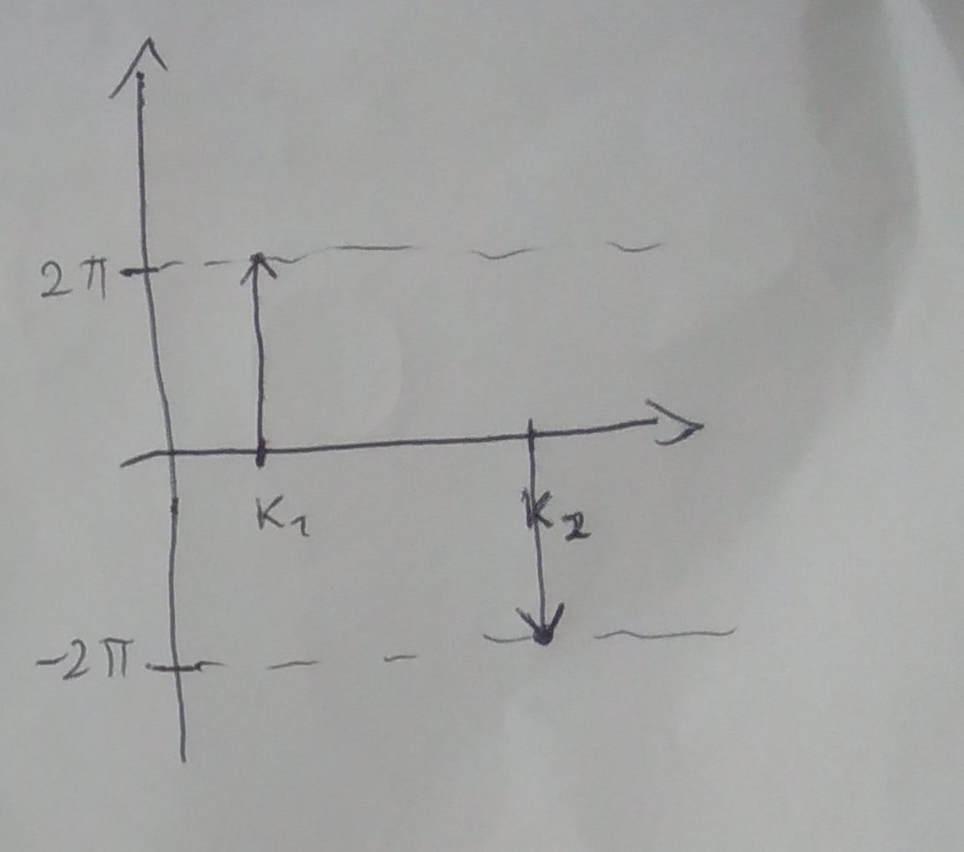
\includegraphics[width=0.5\textwidth]{./rysunki/jpg/zmo.jpg} \\
W przypadku kwadratu wszędzie wynosi zero. \\
Zatem faktycznie nie da się rozciąć pierścienia i złożyć z niego kwadratu. \\
Znakowana miara obłości pokrywa wszystkie naturalne przykłady (tzn. takie, które wymyśliłem, zanim 
starałem
się wymyśleć takie, które ją obalą). W szczególności potrafi nie tylko rozróżnić, ale i 
sklasyfikować
wszystkie figury o brzegach składających się z odcinków i łuków (co pokażemy w następnym 
rozdziale). \\
I tutaj zbliżamy się do problemu - idealny niezmiennik pozwalałby nie tylko na określenie czy dane 
dwie figury nie są równoważne przez cięcia. Wynikało by też z niego, że jeśli jest równy dla obu 
figur, to są one równoważne. Przy definiowaniu niezmienników jako własności 
brzegu wymaga to jednak chociażby
faktu, że jeśli brzegi są sobie (w pewnym sensie jaki ściśle za niedługo podamy) równoważne przez 
cięcia,
to figury także. Na szczęście okaże się, że tak jest. \\
W kolejnych rozdziałach zajmiemy się właśnie szukaniem takiego twierdzenia odwrotnego (czy właściwie
działającego w obie strony) i związanego z nim niezmiennika. Zakończy się to dyskusją, czy wyniki 
nas
satysfakcjonują. \\
Pokażemy też w międzyczasie, że znakowana miara obłości takim niezmiennikiem nie jest (chociaż jest 
nim
dla figur o brzegach składających się z odcinków i łuków).
% Ale najpierw sformalizujmy nieco nasze pojęcia.
\section{Formalizacja pojęć}
%Najpierw sformalizujmy nieco nasze pojęcia. \\
%Sformalizujemy teraz nieco nasze poję
Zajmujemy się zwartymi figurami w $\mathbb{R}^2$, których brzegi są skończonymi zbiorami 
 rozłącznych 
obrazów
prostych krzywych
zamkniętych, kawałkami $C^\infty$.
Wszędzie dalej kiedy będzie użyte słowo figura, będzie to oznaczało właśnie taki podzbiór 
$\mathbb{R}
^2$. \\
Ponadto wszystkie krzywe parametryzujemy ich długością.
\subsection{Krzywa z wyróżnioną stroną}
%\todo{poprawić}
Krzywa z wyróżnioną stroną będzie to krzywa wraz z wybraną jedną z dwóch klas rodzin ciągłych cięć 
 pewnych wybranych
 podwiązek wiązki stycznej $\mathbb{R}^2$ zawieszonej nad $C^\infty$ fragmentami tej krzywej. \\
Dla krzywej $\gamma : [a, b] \to \mathbb{R}^2$ patrzymy się na rodzinę podwiązek wiązki stycznej
$\mathbb{R}^2$ złożoną z podwiązek zawieszonych nad kolejnymi  
$C^\infty$ fragmentami krzwej, złożonych
z dowolnych podprzestrzeni dopełniczych do podprzestrzeni rozpinanych przez wektory styczne.
% (na rogach wybieramy tak, by przestrzeń była dopełnicza dla obu wektorów stycznych). 
\\
Dla takiej rodziny podwiązek wybieramy teraz ciągłe, nieznikające cięcia tych wiązek, 
takie, aby w punktach nieróżniczkowalności
wyznacznik macierzy złożonej z wybranego wektora i z wektora stycznego miał taki sam znak dla obydwu
$C^\infty$ fragmentów. \\
% \rysunek{}
\includegraphics[width=\textwidth]{./rysunki/jpg/wybor_wektorow.jpg} \\
%\smalltodoII{Może ująć to w lemat:}
\textbf{Lemat.} 
%\begin{lemme} 
\textit{Takie rodziny cięć dzielą się na dwie klasy: \\
-rodziny cięć, gdzie w każdym punkcie wyznacznik macierzy [wektor styczny, wektor z odpowiedniego 
cięcia] jest dodatni 
oraz\\
-rodziny cięć, gdzie w każdym punkcie wyznacznik macierzy [wektor styczny, wektor z odpowiedniego 
cięcia] jest ujemny. \\}
%\end{lemma}
\textbf{Dowód.}
Rodziny cięć są rodzinami ciągłych cięć jednowymiarowych wiązek, wyznacznik jest ciągły oraz
zależność wektora stycznego od parametru jest ciągła. Z wyboru cięć, w punktach 
nieróżniczkowalności, wyznacznik nie zmienia znaku. Stąd jeżeli wyznacznik zmieniałby znak w 
 obrębie 
rodziny cięć, 
musiałby zmieniać znak we wnętrzu
różniczkowalnej krzywej, ale wtedy w pewnym momencie zerowałby się, co oznaczałoby, że cięcie znika.
Sprzeczność. Stąd wyznacznik nie zmienia znaku w obrębie rodziny cięć. $_\square$\\
Wybór jednej z rodzin klas takich cięć nazywamy wyborem strony krzywej. Ma to oddawać 
koncept oznaczany graficznie zazwyczaj w taki sposób: \\
%\\ \smalltodoII{koncept oznaczany graficznie zazwyczaj w taki sposób XD:}
% \rysunek{}
\includegraphics[width=\textwidth]{./rysunki/jpg/ma_oddawac_cos_takiego.jpg} \\
Zauważmy, że dla figury rozpatrywanej jako dwuwymiarowa rozmaitość oraz komponenty jej brzegu jedna 
z tych
klas jest złożona z rodzin złożonych z cięć złożonych z wektorów leżących w wiązce stycznej do tej 
rozmaitości, a druga, z rodzin złożonych z cięć złożonych z wektorów do 
niej
nienależących. Ponieważ dla każdej komponenty parametryzację możemy wybrać niezależnie, więc da się 
je wybrać
tak, by jedna z tych klas odpowiadała dla wszystkich komponent wnętrzu rozmaitości. Od tej pory 
będziemy
zakładali taki właśnie wybór parametryzacji. Co więcej taki, by strona z 
%ujemnym 
dodatnim wyznacznikiem była 
we wnętrzu.
% (Czyli obiegamy figury przeciwnie do ruchu wskazówek zegra).
\\
Od tej pory o wszystkich krzywych zakładamy, że mają wyróżnioną stronę.
Przyjmujmy, że dla wszystkich figur omawianych w pracy wyróżniona strona brzegu figury odpowiada 
wnętrzu figury. \\
Funkcję krzywizny ze znakiem $k^\pm$ określamy na podstawie funkcji krzywizny krzywej $k$ tak, że 
jeśli w danym punkcie wyznacznik 
macierzy [wektor styczny, wektor 
drugiej pochodnej] 
ma ten
sam znak co wybrana klasa, to $k^\pm = k$, w przeciwnym wypadku $k^\pm = -k$.
\section{Poszukiwanie twierdzenia odwrotnego} 

\subsection{Równoważność z problemem na brzegach}
Najpierw dowiedziemy, że zagadnienie równoważności takich figur przez cięcia jest równoważne 
równoważności
przez cięcia ich brzegów w następującym sensie: \\
Powiemy, że dwie krzywe są równoważne przez cięcia, jeżeli obraz jednej z nich można pociąć i za 
pomocą
izometrii przekształcić na obraz drugiej (zachowując wyróżnioną stronę), 
przy czym dopuszczamy cięcia pustej
przestrzeni na dwie
odpowiadające sobie krzywe oraz sklejanie takich krzywych: \\
% \rysunek{słynne rysunki rozcinania pustej przestrzeni oraz klejenia dwóch odpowiadających krzywych
% dopiski - kreacja, anihilacja}
\includegraphics[width=\textwidth]{./rysunki/jpg/kreacja.jpg} \\
\includegraphics[width=\textwidth]{./rysunki/jpg/anihilacja.jpg} \\
\textbf{Uwaga techniczna}\\
Teraz zostanie omówiony przypadek, kiedy żadne dwa sąsiednie $C^\infty$ fragmenty krzywych nie 
spotykając się pod kątem $180\si{\degree}$. Oznacza to, że nie tworzą następujących konfiguracji 
(nazywanych dalej szpicami, odpowiednio, wypukłym i wklęsłym): \\
\includegraphics[width=\textwidth]{./rysunki/jpg/szpice.jpg}
Następnie (\ref{Redukcja szpiców}) zostanie omówiona redukcja przypadku ze szpicami do przypadku 
 bez 
szpiców. \\
\textbf{Implikacja w jedną stronę:} \\
\textit{,,Jeśli brzegi figur są równoważne, a figury mają równe pola, to figury również są
 równoważne.''} \\
Weźmy dwie figury $A$ oraz $B$ o równych polach, takie, że brzegi są równoważne przez cięcia. Niech 
cięcie
to będzie realizowane poprzez podział brzegu $A$ i przekształcenie jego fragmentów przez izometrie
 płaszczyzny oraz,
jeśli konieczny, podział ,,pustej przestrzeni'' na krzywe i anihilację pasujących krzywych tak jak 
opisane
wyżej. Niech ta operacja świadcząca o równoważności dwóch brzegów przez cięcia nazywa się $\phi$. \\
Skonstruujemy teraz redukcję problemu podziału tych figur do problemu podziału wielokątów, który, 
jak wiadomo
 z twierdzenia Wallace–Bolyai–Gerwien'a \cite{WBG}, zawsze ma rozwiązanie. \\
Rozpatrzmy fragmenty na które podzielony jest brzeg $A$. Każdy z nich jest zbiorem zwartym, więc
(za wyjątkiem sąsiadujących) jest on w niezerowej odległości od pozostałych fragmentów. Dla tych, 
których
 obraz przez $\phi$ jest w $B$ (to znaczy, że fragment nie został zanihilowany z mu odpowiadającym)
 jest on również w niezerowej odległości od wszystkich fragmentów (za wyjątkiem tych z którymi ma 
 wspólne
 końce) z których został ułożony brzeg $B$ przy  użyciu $\phi$.  \\
Fragmentów jest skończenie wiele, niech więc $\varepsilon$ będzie dodatnią liczbą rzeczywistą 
mniejszą
od wszystkich tych odległości dla wszystkich par niesąsiadujących fragmentów. \\
rozpatrzmy $\frac{\varepsilon}{4}$-owe otoczki wszystkich fragmentów krzywej. W każdym z tych 
fragmentów
prowadzimy
łamaną prostą o początku i końcu w końcach fragmentu taką, że pierwsza i ostatnia krawędź łamanej
\label{180 stopni} spełnia
następujący warunek na kąty względem wektorów stycznych (zarówno w $A$, jak i w $B$): \\
% \rysunek{początek i koniec łamanej, dwusieczna kąta  z wektorów stycznych}
\includegraphics[width=\textwidth]{./rysunki/jpg/konce_lamanej.jpg} \\ % początek i koniec łamanej
% \rysunek{przypadek 180 stopni}
Tutaj właśnie korzystamy z chwilowego założenia, że żadne dwa sąsiednie $C^\infty$ fragmenty 
 krzywej 
nie spotykają się pod kątem $180\si{\degree}$. \\
Wtedy wszystkie obszary ograniczone przez fragmenty krzywej oraz łamane w odpowiadających im
otoczkach oraz ich obrazy przez $\phi$ są parami rozłączne za wyjątkiem końców fragmentów dla
sąsiadujących fragmentów. \\
Możemy odciąć je z $A$ i przerzucić w odpowiednie miejsca na $B$. \\
%Fragmenty brzegu $A$, które się z sobą zanihilują, odcinamy po jednym z pary wraz z jego łamaną i
%anihilujemy. \\
Fragmenty brzegu $A$, które się z sobą zanihilują, odcinamy parami wraz z ich łamanymi i
anihilujemy. \\
% \rysunek{anihilecja}
\includegraphics[width=\textwidth]{./rysunki/jpg/przeksztalcenie_A_A'_2_1.jpg} \\
Niech $A'$ oznacza tak powstałą z $A$ figurę (jak widać na rysunku niekoniecznie spójną).
Brzeg $B$ dzieli się na dwa obszary - fragmenty pochodzące z fragmentów brzegu $A$ oraz fragmenty
pochodzące z rozcięć przestrzeni.
Pozostaje ,,obsłużyć'' fragmenty brzegu $B$ pochodzące z kreacji krzywych z przestrzeni. \\
Potrzebny będzie następujący lemat:
\begin{lemma}\label{lemat o dzieleniu}
    Dla dowolnej krzywej $\gamma : [a, b] \to \mathbb{R}$ takiej jak tu przyjmujemy i dowolnego 
    dysku
    $\mathcal{O}$ zawartego w $\mathbb{R}^2$ da się znaleźć taki podział $\gamma$, by poprzez
    izometrie płaszczyzny
    dało się go odwzorować we wnętrze $\mathcal{O}$ tak, że obrazy fragmentów będą parami rozłączne.
\end{lemma}
\noindent\textbf{Dowód.}
Dla dysku $\mathcal{O}$ przez $d(\mathcal{O}$) oznaczamy średnicę dysku. Dla krzywej $\gamma$ 
przez $l(\gamma)$ oznaczamy długość krzywej.
% Obłość $\gamma$ jest skończona, zatem skończona jest obłość każdego fragmentu $\gamma$.
Konstuujemy ciąg podziałów $\gamma$
tak, by dla każdego $n$ w $n$-tym podziale
% obłość każdego fragmentu była mniejsza niż $\pi/2^n$ oraz by
długość każdego fragmentu była mniejsza niż $d(\mathcal{O})/(2n+1)$ ale (poza, być może, 
ostatnim)
większa niż $d(\mathcal{O})/(2n+3)$. \\
%\smalltodoII{dać lepsze oznaczenia}
Fragmentów tych będzie co najwyżej część całkowita z $\frac{l(\gamma)}{d(\mathcal{O})/(2n+3)}$,
czyli część całkowita z $(2n+3)\frac{l(\gamma)}{d(\mathcal{O})}$. Każdy z tych fragmentów zmieści 
 się w dysku
o średnicy $d(\mathcal{O})/(2n+1)$. Kół o średnicach $d(\mathcal{O})/(2n+1)$ w kole $\mathcal{O}
$ da się
na pewno zmieścić co najmniej $6\frac{n(n+1)}{2}+1$. \\
% \rysunek{sześciokąty}
\includegraphics[width=\textwidth]{./rysunki/jpg/szesciokaty.jpg} \\
Dla $n$ takiego że $3\frac{n(n+1)+1}{2n+3}>\frac{l(\gamma)}{d(\mathcal{O})}$, krzywa zmieści 
się
rozłącznie w okręgu dla podziału odpowiadającego $n$. $_\square$
% \begin{lemma}
%     Dla każdego takiego podziału krzywa zmieści się w kole o promieniu $a$.
% \end{lemma}
% \begin{proof}
%
% \end{proof}


Bierzemy wszystkie krzywe (bez wyróżnionej strony) z których powstały te fragmenty brzegu $B$ 
poprzez kreację, 
łączymy je
w jedną długą krzywą prostą (jeśli trzeba to łamiemy je, żeby zachować warunek "prostości").
Tak skonstruowaną krzywą umieszczamy (dokonując cięć również we wszystkich miejscach uprzednich 
łączeń) w kole tak małym, by było zawarte we wnętrzu $A'$ tak jak mówi 
lemat \ref{lemat o dzieleniu}. \\
\includegraphics[width=\textwidth]{./rysunki/jpg/krzywa_w_szesciokacie_2_1.jpg} \\
Przy czym zagęszczamy podział tak mocno by obłość każdego fragmentu nie
przekraczała $\pi/8$ 
%oraz by 
długość żadnego fragmentu nie była większa niż $\varepsilon/8$ oraz 
by żaden fragment (o ile nie jest odcinkiem) nie miał w żadnym punkcie zerowej wartości krzywizny 
(w celu spełnienia ostatniego warunku dodajemy punkty cięć na końcach fragmentów będących 
odcinkami oraz w punktach izolowanych zbioru punktów gdzie krzywizna ma wartość $0$). \\
Należy teraz wykonać następujące cięcia w $A'$ (okręgi narysowane są tylko w celach 
pomocniczych i nie przedstawiają cięć): \\
% \rysunek{jak ciąć}
\includegraphics[width=\textwidth]{./rysunki/jpg/jak_ciac_3_1.jpg} \\
% \rysunek{jak ciąć w środku kulki}
Dyski rozmieszczamy tak, by tworzyły koncentryczne sześciokąty. Wyróżnijmy punkt $o$, który jest 
środkiem symetrii powstałej figury. Kiedy będziemy mówili ,,radialnie'', bądź ,,wzdłóż promienia'' 
będziemy mieli na myśli kierunki radialne względem tego punktu. \\
Wszystkie fragmenty krzywej umieszczamy w dyskach (poza centralnym) tak, by wektory do nich styczne 
 na końcach 
tworzyły kąt co do modułu mniejszy niż $\frac{\pi}{8}$ z promieniem przechodzącym przez środek 
dysku w którym się znajdują. Fragment znajdujący się w centralnym dysku umieszczamy dowolnie, ale 
 tak, by jeden jego koniec był bliżej $o$ niż drugi. Z 
warunku ograniczającego obłość fragmentów do $\frac{\pi}{8}$ 
otrzymujemy, że dla każdego fragmentu jeden jego koniec leży bliżej $o$ niż drugi. 
Niech $B$ oznacza zbiór końców kawałków krzywych bliższych $o$, za to $D$ zbiór końców 
kawałków krzywych dalszych od $o$. Łączymy teraz elementy z $B$ oraz elementy z $D$ łamanymi 
według schematu pokazanego na powyższym rysunku. Te łamane oraz fragmenty krzywych są liniami cięć. 
\\
\noindent Z powyższych fragmentów układamy odpowiednie fragmenty brzegu $B$. \\
Tak powstała figura $A''$ jest sumą rozłączną wielokątów. Niepokryta część $B$ jest wielokątem,
nazwijmy ją $B''$. $A$ oraz $B$ miały równe pola, więc $A''$ i $B''$ również mają równe pola.
Są więc równoważne przez cięcia, więc $A$ i $B$ również są. \\[8pt]
\noindent \textbf{Implikacja w drugą stronę:} \\
\textit{,,Jeśli figury są równoważne, to ich brzegi również są równoważne''}. \\
Podział figur $A$, $B$ zadaje równoważność brzegu $A$ z sumą brzegów fragmentów na jakie została 
 pocięta $A$
oraz równoważność tej sumy brzegów z brzegiem $B$. Stąd dla równoważnych figur ich brzegi również 
są
równoważne.
$_\square$ 
%\\
\subsubsection{Redukcja przypadku ze szpicami}\label{Redukcja szpiców}
\textbf{Szpic wypukły}\\
Zaczynamy od znalezienia dysku o małym promieniu zawartego w figurze. Wycinamy z niego fragment 
zawierający jako brzeg krzywą identyczną z początkiem jednej z krzywych tworzących szpic, ale 
o przeciwnej wyróżnionej stronie i przyklejamy go do szpicu. Proces ten schematycznie 
ilustruje rysunek: \\
\includegraphics[width=\textwidth]{./rysunki/jpg/szpic_wypukly_radzenie_sobie.jpg} \\
%\todo{to trzeba narysować}
\noindent\textbf{Szpic wklęsły}\\
W przypadku szpicu wklęsłego wycinamy fragment figury zawierający jako brzeg początek jednej z 
krzywych tworzących szpic i przenosimy go w inne miejsce płaszczyzny (poza figurę). 
Proces ten schematycznie ilustruje rysunek: \\
\includegraphics[width=\textwidth]{./rysunki/jpg/szpic_wklesly_radzenie_sobie.jpg} 
%\\
\subsection{Kiedy ZMO zawodzi}
Pokazaliśmy, że rozstrzygając równoważność przez podział figur o tym samym polu wystarczy 
rozstrzygnąć
równoważność przez podział ich brzegów. Zastanówmy się, czy znakowana miara obłości jest 
wystarczającym
kryterium do klasyfikacji krzywych - tzn. czy dowolne dwie nierównoważne mają różną oraz czy dowolne
dwie równoważne mają taką samą. \\
W \ref{ZMO} odpowiedzieliśmy sobie twierdząco na drugie pytanie.
% Pokażemy teraz, że odpowiedź na pierwsze
% pytanie jest twierdząca dla krzywych złożonych wyłącznie z łuków i odcinków.
Odpowiedź na pierwsze pytanie jest twierdząca dla krzywych złożonych wyłącznie z łuków i odcinków.
Mając tą samą znakowaną miarę obłości mają tą samą sumaryczną długość łuków okręgów o odpowiednich
promieniach z wyróżnioną stroną z odpowiedniej strony. Fragmenty te można kleić ze sobą i ciąć, tak 
by
z jednej krzywej otrzymać drugą. Fragmenty o krzywiźnie 0 można dowolnie kreować i anihilować. \\
Znakowana miara obłości nie potrafi jednak rozróżnić wszystkich nieprzystających do siebie przez 
cięcia
krzywych. Skonstruujemy tego przykład. Najpierw jednak przeprowadzimy analizę czym jest
wprowadzona tutaj znakowana miara obłości i jak ma się do krzywizny krzywej.
\subsubsection{Jak wygląda znakowana miara obłości}
 Niech $k(t)$ będzie funkcją krzywizny od czasu jakim 
% krzywa
jest
sparametryzowana.
Rozpatrzmy krzywą o ściśle monotonicznej krzywiźnie ($\forall_t\ k'(t) \neq 0$) dla
%Dla takich krzywych 
których znak znakowanej krzywizny jest stały. Rozpatrzmy najpierw przypadek, gdzie 
$k^\pm = k$.
\\
% Niech $k(t)$ będzie funkcją krzywizny od czasu jakim 
%% krzywa
%jest
%sparametryzowana.
 Ze ścisłej monotoniczności istnieje funkcja odwrotna $t(k) : [k_\text{MIN}, 
k_\text{MAX}]
\to \mathbb{R}$, która mówi w jakiej chwili czasu uzyskana była dana wartość krzywizny. \\
Wyrazimy teraz znakowaną miarę obłości takiej krzywej poprzez jej krzywiznę oraz na odwrót - jej 
krzywiznę
poprzez jej znakowaną miarę obłości. \\
\begin{lemma}
    Dla krzywej z wyróżnioną stroną o ściśle rosnącej krzywiźnie takiej, że 
    $k^\pm = k$ jej ZMO ma gęstość.
\end{lemma}
\begin{proof}
    Z definicji znakowanej miary obłości (\ref{ZMO_def}) oraz założenia, że $k^\pm = k$, dla
     dowolnego przedziału $[k_1, k_2]$ jest ona równa:
    \begin{equation}
        \mu_O([k_1, k_2]) = \displaystyle\int\limits_{t(k_1)}^{t(k_2)}k(t)\ \text{d}t
    \end{equation}
    Co przez zamianę zmiennych jest równe:
    \begin{equation}
        \displaystyle\int\limits_{t(k_1)}^{t(k_2)}k(t)\ \text{d}t =
        \displaystyle\int\limits_{k_1}^{k_2}\frac{k}{k'(t(k))}\ \text{d}k
    \end{equation}
    Stąd
    \begin{equation}
    \varrho_O(k) = \frac{k}{k'(t(k))}
    \end{equation} jest szukaną gęstością miary $\mu_K$.
\end{proof}
W ten sposób dla takiej klasy krzywych wyraziliśmy gęstość ich ZMO poprzez ich krzywiznę. Dla 
krzywych bez
łuków, takiej że $\forall_t\ k'(t) \neq 0$, również mamy, że $\mu_K$ 
%również 
ma gęstość, jest ona wtedy sumą gęstości jej składowych o ściśle monotonicznej
krzywiźnie.
Jest tak ponieważ definiujemy tę miarę poprzez całkę, która jest operatorem liniowym. 
\\
%\smalltodoII{określić jakie trzeba przyjąć warunki początkowe}
%\smalltodoII{no takie, ze początek to granica gdzie miara ma gęstość}
%Możemy wyrazić krzywiznę krzywej o ściśle monotonicznej krzywiźnie na podstawie jej ZMO 
 rozwiązując 
%równanie
%różniczkowe:
%\begin{equation}
%    \varrho_O(k(t)) = \frac{k(t)}{k'(t)}\label{kZMO}
%\end{equation}
%o warunku początkowym $k(t_0) = k_0$, gdzie $k_0$ to, w zależności, czy krzywizna krzywej jest 
%ściśle rosnąca, czy ściśle malejąca, odpowiednio najmniejsza bądź największa krzywizna dla której 
%gęstość miary ma niezerową wartość. \\
%Najpierw wyznaczamy zależność $t$ od $k$ jest to:
%\begin{equation}
%t(k) = \int_{k_0}^{k(t)} \frac{\varrho_O(k)}{k} d\ksi- t_0
%\end{equation}
%Jego rozwiązaniem jest:
%\begin{equation}
%    k(t) = k_0e^{\int_{t(k_0)}^{t}\frac{1}{\varrho_O(k(w))}\text{d}w}
%\end{equation}
Dla przypadku, gdzie $k^\pm = -k$ otrzymana zależność to:
\begin{align}
    \varrho_O(k) &= -\frac{k}{k'(t(k))}.\ \
%    % \varrho_K(t) &= -\frac{k(t)}{k'(t)}\
%    \textrm{oraz} \\
%    k(t) &= k_0e^{\int_{t(k_0)}^{t}-\frac{1}{\varrho_O(k(w))}\text{d}w}.
\end{align}
%Jako, że w obydwu przypadkach znakowana krzywizna ma stały znak, możemy odtworzyć również 
 wyróżnioną 
%stronę
%krzywej - w pierwszym przypadku jest to 
%strona której reprezentantem są wektory II pochodnej. 
%W drugim
%przypadku - wektory do nich przeciwne. \\
%Dla krzywych o monotonicznej krzywiźnie, mając ZMO, przypadki $k^\pm = k$ i $k^\pm = -k$ 
%rozróżniamy patrząc na znak 
%gęstości ZMO, 
%w pierwszym przypadku jest ona nieujemna, w drugim - niedodatnia.
\subsubsection{Wnioski płynące z jawnej postaci znakowanej miary obłości}
Krzywa będąca konkatenają dwóch krzywych o ściśle rosnącej krzywiźnie o mierze obłości: \\
% \rysunek{}
\includegraphics[width=0.5\textwidth]{./rysunki/jpg/polowkowa_krzywizna.jpg} \\
każda, ma tą samą miarę obłości co krzywa o ściśle rosnącej krzywiźnie i mierze obłości: \\
% \rysunek{}
\includegraphics[width=0.5\textwidth]{./rysunki/jpg/calkowita_krzywizna.jpg}. \\
Nie są one jednak równoważne przez cięcia. 
%Przyjmujemy, że obydwie krzywe mają wyróżnioną stronę po stronie wektora drugiej pochodnej. \\
%Można to zaargumentować na dwa sposoby. \\
%Sposób pierwszy: \\
 
%Sposób drugi: \\
%Dla dowolnej ustalonej wartości krzywizny $k$ mają one różne
%wartości pochodnej tej krzywizny - zgodnie z (\ref{kZMO}), odpowiednio $2k$ oraz $k$. 
%A pochodna krzywizny dla punktu o danej krzywiźnie nie zmienia się przez cięcia, izometrie ani 
%sklejenia.
\noindent Możemy to zaobserwować wprowadzając następujący niezmiennik: \\
\textbf{Lemat. }\textit{Dla danej wartości krzywizny $k$, jeżeli podczas transformacji danej 
 krzywej $\gamma$ przez cięcia,
 klejenia, 
izometrie, 
kreacje oraz anihilacje żadne cięcie ani klejenie nie było prowadzone przez punkt o 
krzywyźnie $k$, to stała jest wartość: }
\begin{gather}\#_{\gamma}(k) = \text{\textit{\#punktów o krzywiźnie k, gdzie wyróżniona strona jest 
wypukła }} -\\
\text{\textit{\#punktów o krzywiźnie k, gdzie wyróżniona strona jest wklęsła
}} \notag.
\end{gather}
\textbf{Dowód.} Jest tak ponieważ, cięcia oraz klejenia nie zmieniają liczby punktów z założenia, 
 że żadne cięcie 
ani klejenie nie było w punkcie o krzywiźnie $k$, izometrie nie zmieniają tej liczby, a
kreacje i anihilacje krzywych, odpowiednio dodają jeden zarówno do odjemnej jak i do odjemnika, 
odejmują 
jeden zarówno od odjemnej jak i od odjemnika, jeżeli wykreowany/zanihilowany fragment krzywej 
 zawiera punkt o krzywiźnie $k$ bądź też nie zmieniają tej liczby punktów. 
%Tak czy siak 
W każdym przypadku
różnica pozostaje niezmieniona. $_\square$\\
%\\[4pt]
%\smalltodoII{napisać dokładniej czemu}. 
%\indent 
Zauważmy jeszcze nastepującą zależność: \\
Ponieważ wszystkich operacji przy przekształcaniu jednej krzywej na drugą jest skończenie wiele, 
to przy każdym sposobie przekształcenia istnieje wartość krzywizny z krzywej, dla której żadne 
cięcie ani klejenie nie jest prowadzone przez punkt o takiej krzywiźnie. Stąd jeżeli dwie 
krzywe $\gamma_1$, $\gamma_2$ mają dla każdej wartości krzywizny (występującej na co najmniej 
jednej z nich) różne wartości $\#_{\gamma_1}(k)$, $\#_{\gamma_2}(k)$, to nie są one równoważne 
przez cięcia. \\
%Gdyby powyższe krzywe były równoważne ze sobą przez cięcia, to wystarczyłoby wybrać wartość 
%krzywizny z punktu, który nie jest końcem przy żadnym cięciu ani klejeniu i nie występuje na końcu 
%żadnej z krzywych. Da się tak zrobić ponieważ wszystkich operacji w przekształceniu jest tylko 
%skończenie wiele. Ale dla takiego punktu wartość $\#(k)$ jest równa $2$ dla pierwszej krzywej 
%i $1$ dla drugiej, bądź $0$ dla pierwszej 
To prowadzi nas do szukanego wniosku: \\
Powyższe, rozważane przez nas krzywe, dla każdej wartości krzywizny $k$ występującej na tych 
krzywych mają wartości wprowadzonego tu niezmiennika równe, odpowiednio, $2$ i $1$. Nie są 
więc równoważne przez cięcia. \\
\\[4pt]
By potrafić odróżnić od siebie istotnie różne krzywe potrzebujemy niezmiennika zawierającego w sobie
informacje o parametryzacji. Należałoby zawrzeć jakoś informacje jak krzywa rozkłada się na krzywe 
 o 
ściśle
monotonicznej krzywiźnie, które już są wyznaczone jednoznacznie (z dokładnością do izometrii 
 płaszczyzny) przez ich ZMO.
Wtedy znalibyśmy rodzinę krzywych z dokładnością do ich cięć i izometrii płaszczyzny.
W następnym rozdziale przedstawimy niezmiennik, który faktycznie jest zachowywany przy cięciach,
izometriach płaszczyzny i
 sklejeniach oraz jest różny dla krzywych (a stąd dla figur) które równoważne nie są.

\subsection{Wielka grupa abelowa}
Niech $\mathcal{A}$ będzie rodziną wszystkich
prostych krzywych, kawałkami $C^\infty$, sparametryzowanych długością z wyróżnioną stroną
(zapisywaną jako $\mathcal{S}(\gamma) = 1$ dla dodatniego wyznacznika oraz $\mathcal{S}
(\gamma)=-1$ dla ujemnego wyznacznika). \\
Rozepnijmy wolna grupę abelową na $\mathcal{A}$. \\
Określmy teraz relacje w tej grupie: \\
-kreacji/anihilacji \\
-cięcia/klejenia \\
-izometrii 
\subsubsection{Kreacja/anihilacja}
Dla $\gamma_1 : [a, b] \to \mathbb{R}^2, \gamma_2 : [c, d] \to \mathbb{R}^2$
\begin{gather}
    \gamma_1[[a,b]]=\gamma_2[[c,d]] \notag\\\land\notag\\
    \Big(\big( \gamma_1(a) = \gamma_2(c) \land \mathcal{S}(\gamma_1)=-\mathcal{S}(\gamma_2)\big) \\
    \lor \notag\\
    \big(\gamma_1(a) = \gamma_2(d) \land \mathcal{S}(\gamma_1)=\mathcal{S}(\gamma_2) \big)\Big)
    \notag\\
     \implies \gamma_1 + \gamma_2 = 0\notag
\end{gather}
\subsubsection{Cięcia/klejenie}
Dla $\gamma_0 : [a_1, a_n] \to \mathbb{R}^2, \gamma_1 : [a_1, a_2] \to \mathbb{R}^2, \ldots, 
\gamma_{n-1} :
[a_{n-1}, a_n] \to \mathbb{R}^2$, takich że $a_1 < a_2 < \ldots < a_{n-1} < a_n$
\begin{gather}
    \big(
    (\forall t \in [a_i, a_{i+1}])\gamma_0(t)=\gamma_i(t)) \land (\forall i)\mathcal{S}(\gamma_0) =
    \mathcal{S}(\gamma_i)
    \big) \\
    \implies \gamma_0 - \gamma_1 - \ldots -\gamma_n = 0\notag
\end{gather}
\subsubsection{Izometrie}
Dla $\gamma_1 : [a, b] \to \mathbb{R}^2, \gamma_2 : [c, d] \to \mathbb{R}^2$
\begin{gather}
    |b-a| = |c-d| \\
    \land \\
    \Big(\big( \forall_{t \in [0, b-a]}k^\pm_{\gamma_1}(a+t) = k^\pm_{\gamma_2}(c+t)
    \land
    \mathcal{S}(\gamma_1)=\mathcal{S}(\gamma_2)\big) \notag\\
    \lor \\
    \big(\forall_{t \in [0, b-a]}k^\pm_{\gamma_1}(a+t) = k^\pm_{\gamma_2}(d-t)
    \land
    \mathcal{S}(\gamma_1)=-\mathcal{S}(\gamma_2)\big)\Big) \notag\\
    \implies \gamma_1 - \gamma_2 = 0\notag
\end{gather}
Odpowiada to odwzorowaniom przez izometrie $\mathbb{R}^2$,
\begin{gather}
    \exists\Lambda_{-\text{izometria}}\ \gamma_1 \equiv \Lambda\circ\gamma_2 \notag\\
    \land \notag\\
    \Big(\big(\det{\Lambda} = 1 \land \mathcal{S}(\gamma_1)=\mathcal{S}(\gamma_2) \big) \\
    \lor \notag\\
    \big(\det{\Lambda} = -1 \land \mathcal{S}(\gamma_1)=-\mathcal{S}(\gamma_2) \big)\Big) \notag\\
    \implies \gamma_1 - \gamma_2 = 0,\notag
\end{gather}
ponieważ funkcja znakowanej krzywizny określa jednoznacznie krzywą (bez wyróżnionej strony)
z dokładnością do jej początku i wektora stycznego w początku~\cite{Spivak}.
%\smalltodoII{napisać równanie różniczkowe}
Dzieje się tak, ponieważ znając funkcję znakowanej krzywizny danej krzywej jesteśmy w stanie 
napisać równianie różniczkowe wiążące pierwszą i drugą pochodną krzywej. \\
\indent Druga pochodna równa się wektor prostopadły do pierwszej dodatnio zorientowany razy 
 znakowana 
krzywizna: \\
\begin{equation}
    \colvect{\gamma''_x(t)}{\gamma''_y(t)} = k^\pm(t)\colvect{-\gamma'_y(t)}{\gamma'_x(t)}
\end{equation}
%\smalltodoII{napisać coś o rozwiązaniu tego równania}
%Można je przedstawić również jako:
Równanie różniczkowe to można przedstawić również jako:
\begin{gather}
\gamma''(t) = \begin{bmatrix}
0 & -k^\pm(t) \\
k^\pm(t) & 0
\end{bmatrix}\gamma'(t)
\end{gather}
Jest to liniowe równanie różniczkowe pierwszego stopnia (ze względu na pochodną krzywej). \\
Dla krzywej $\gamma : [a, b] \to \mathbb{R}^2$, dla warunku początkowego $\gamma'(t_0)=\gamma'_0 = 
\colvect{{\gamma'_0}_x}{{\gamma'_0}_y}$ jego rozwiązaniem jest wtedy:
%\todo{napisać to rozwiązanie}
\begin{gather}
\gamma'(t) = \notag \\ 
-\begin{pmatrix}\cos\left(\int_a^t k^\pm(w)\  \text{d}w\right) & 
\sin\left(\int_a^t k^\pm(w)\  \text{d}w\right) \\
-\sin\left(\int_a^t k^\pm(w)\  \text{d}w\right) & \cos\left(\int_a^t k^\pm(w)\  \text{d} w\right)
\end{pmatrix} \colvect{{\gamma'_0}_x}{{\gamma'_0}_y} \\
 = -\colvect{{\gamma'_0}_x \cos\left(\int_a^t k^\pm(w)\  \text{d}w\right) + {\gamma'_0}_y 
\sin\left(\int_a^t k^\pm(w)\  \text{d}w\right)}{{\gamma'_0}_y \cos\left(\int_a^t k^\pm(w)\  \text{d}
w\right) - {\gamma'_0}_x \sin\left(\int_a^t k^\pm(w)\  \text{d}w\right)} \notag
\end{gather}
%Krzywą $\gamma$ możemy otworzyć z jej pochodnej rozwiązując równanie różniczkowe.
Dla warunku początkowego $\gamma(0) = \gamma_0 = \colvect{{\gamma_0}_x}{{\gamma_0}_y}$, krzywa 
 gamma 
jest to
\begin{gather}
\gamma(t) = \gamma_0 + \int_a^t \gamma'(w) \  \text{d}w
\end{gather}
%Dla warunku początkowego $\gamma $
\\[16pt]
\indent Zauważmy również, że trzecia relacja utożsamia również krzywe o tym samym obrazie, a różnej 
 parametryzacji ze
względu na przedział którym są sparametryzowane. \\
\indent Przez wielką grupę abelową (nazywaną dalej WGA) rozumiemy grupę ilorazową powstałą przez 
wydzielenie wolnej grupy abelowej rozpiętej na $\mathcal{A}$ przez relacje kreacji/anihilacji, 
cięcia/klejenia oraz izometrii.
\subsubsection{Równoważność elementu w wielkiej grupie abelowej z klasą 
%figur 
krzywych równoważnych ze sobą przez 
cięcia}
%Widać \\
%\todo{Może jednak trochę dokładniej}
%Dowiedziemy, że element WGA odpowiada jednej klasie 
\textbf{Twierdzenie. } \\
\textit{Dwie kawałkami $C^\infty$, proste krzywe sparametryzowane długością z wyróżnioną stroną 
są ze sobą równoważne przez cięcia wtedy i tylko wtedy, gdy odpowiada im ten sam element w WGA.} \\
\textbf{Dowód.} \\
\textbf{Implikacja w jedną stronę:}\\ 
%Ustalmy liczbę rzeczywistą $r$ oraz 
Weźmy element z WGA. Pokażemy, że odpowiada mu dokładnie 
 jedna klasa równoważności przez cięcia
%figur.
krzywych.
\\
Jeśli odpowiadałyby dwie, to biorę po reprezentancie każdej z nich i patrzę na ich elementy w 
niewydzielonej
grupie. Elementy te z założenia przechodzą na ten sam element przez odwzorowanie ilorazowe.  
%tym samym w wydzielonej, więc te relacje jakoś je zwijają. \\
Stąd istnieje ciąg relacji $\psi$ z grupy ilorazowej pozwalający przekształcić wyrażenie
 odpowiadające 
pierwszej krzywej w wyrażenie odpowiadające drugiej krzywej.
Ciąg przekształceń złożony z przekształceń odpowiadających kolejnym relacjom 
z $\psi$ stanowi o równoważności krzywych. \\
% To senioeoofaja cięcoa. {onadfoeofe możena z zauważeć , zę w pownem momecicie zacząłem pisać 
%całkowicie verz
% patrzenia na klawoateurę
% po odzie rto znacznoe lieoaj nież się zspodzieawałem. zSz czełdó lnei ż e staeałen się apasiasć 
%wiraen sirwas
%  sdioasgsi c szir czo0od aifa naiej fpsijiakdf/ nke.
\textbf{Implikacja w drugą stronę:} \\
Analogicznie: \\
Jeśli dwie krzywe $\gamma_1$, $\gamma_2$ są równoważne, to istnieje ciąg transformacji $\phi$ przez 
 izometrie oraz kreacje/
anihilacje przekształcający jedną krzywą na drugą. \\
Ciąg relacji złożony z relacji odpowiadających transformacjom z $\phi$ pozwala przekształcić 
element w niewydzielonej grupie odpowiadający $\gamma_1$ w element odpowiadający $\gamma_2$. 
Stąd te elementy mają jednakowy obraz przez odwzorowanie ilorazowe. Obu krzywym 
odpowiada, więc ten sam element WGA. $_\square$
\subsubsection{Dyskusja, że to niewiele daje}
Niezmiennik jakim jest element w WGA faktycznie daje charakteryzację. Jednak jego wyznaczenie (bądź 
w 
ogóle
opisanie) nie wydaje się łatwiejsze niż rozstrzygnięcie problemu dla danych figur bez tego aparatu
pojęciowego. Wiedza o możliwości przedstawienia tego problemu w postaci WGA nie dała mi żadnej 
odpowiedzi
na żadne pytanie postaci ,,opisuję jakoś dwie figury, chcę rozstrzygnąć, czy są równoważne przez 
cięcia'',
którego nie potrafiłbym rozstrzygnąć w inny sposób. Opis ten daje jednak inne rzeczy.\\
Odzwierciedliliśmy bowiem problem w strukturę grupową. Zrobiliśmy to również w taki sposób, że 
każdej klasie
figur równoważnych przez cięcia odpowiada jeden element w grupie abelowej oraz liczba rzeczywista 
(pole)
oraz każdemu elementowi z grupy wraz z liczbą z zakresu $(0, \infty)$ (możliwe pola, bo tnąc zawsze 
można
zejść dowolnie blisko zera ,,redukując kąt zataczany przez krzywe i zbliżając powstałe krawędzie'', 
a
kreując krzywe można uzyskać dla wybranej klasy dowolnie duże pole) \\
% \rysunek{redukcja krzywizny}
\includegraphics[width=\textwidth]{./rysunki/jpg/wonsz.jpg} \\
odpowiada jedna klasa figur równoważnych przez podział. \\
Załóżmy teraz, ze chcemy określić pewien niezmiennik, prostszy w wyliczeniu, ale taki, że jego 
możliwe wyniki
nadal będą w bijekcji z klasami podziału. Załóżmy ponadto, że przeciwdziedzina tego niezmiennika 
będzie miała
strukturę grupową. Jest to dość naturalne założenie, pierwsze dwa naturalne niezmienniki jakie 
wprowadziliśmy, mianowicie obłość i znakowana miara obłości, miały tę strukturę, a niezmienniki 
 były 
homomorfizmami,
gdzie po jednej stronie działaniem było wzięcie na raz dwóch krzywych (albo, można myśleć, ich 
konkatenacja),
a po drugiej stronie - suma ich niezmienników. \\
Wydaje się, że jeśli niezmiennik wyrażony w czymś o strukturze grupowej miałby się zachowywać 
,,przyzwoicie''
powinien mieć tę własność. Mając jednak naszą WGA widzimy, że każdy taki niezmiennik pozwalający na
rozróżnianie dwóch dowolnych klas 
%oraz nie mający ??????? 
będzie miał zanurzoną w sobie WGA, w tym sensie 
będzie
nieprostszy. \\
Oczywiście nie wykluczam, że nie spostrzegłem jakiś metod rozróżniania klas figur przy użyciu 
 innego 
typu
niezmienników bądź bez określania niezmienników w ogóle. Może też istnieje efektywna metoda 
 określania
jednakowości elementów w WGA. Podejrzewam też, że przy innym spojrzeniu możliwe byłoby napisanie 
niezmiennika, który lepiej charakteryzowałby krzywe (lub nawet charakteryzował je w pełni) i 
był w jakiś sposób (przynajmniej dla pewnej klasy krzywych) wyliczalny. Być może byłby on nawet 
równoważny WGA, ale dzięki innemu podejściu do problemu może sytuacja byłaby jaśniejsza. 
Możliwe, ze powiedziało by to też coś wtedy o strukturze samej WGA. Jednak na ten moment żadne 
z powyższych nie zostało przeze mnie znalezione.
% pewnego zakresu charakterystycznego dla tego elementu (możliwe pola)

\section{Uwaga o topologii}
Na zbiorze figur takich jak omawiane w tej pracy, branych z dokładnością do izometrii na
płaszczyźnie można określić odległość między nimi jako infimum pola różnicy symetrycznej brane po 
wszystkich
reprezentantach klas (czyli po wszystkich obrazach izometrii na płaszczyźnie). \\ 
Różnicę symetryczną zbiorów $A$ i $B$ będziemy oznaczać przez $A \triangle B$. \\
Pole figury $f$ będziemy oznaczać przez $\mathcal{P}(f)$. \\
\indent Zauważmy, że mając daną figurę $A$, przestrzeń położeń innej figury $B$ względem $A$ 
zawierającą wszystkie położenia o różnicy symetrycznej o polu mniejszym niż $\mathcal{P}(A) 
+ \mathcal{P}(B)$ da 
się sparametryzować zbiorem zwartym $D^2 \times S^1 \times S^0$. \\ 
\indent W tym celu wyróżniamy punkt $b \in B$. Kiedy $b$ leży poza dyskiem (o odpowiednio dużym 
promieniu) pole powierzchni różnicy symetrycznej $A \triangle B$ tak położonych figur $A$ i $B$ 
jest równe $\mathcal{P}(A) + \mathcal{P}(B)$. Parametryzujemy 
ten dysk dyskiem $D^2$. Dla każdego położenia punktu $b$ położenie figury jest zdeterminowane 
przez jej obrót (co parametryzujemy przez $S^1$) i symetryczne odbicie (co parametryzujemy 
przez $S^0$). Parametryzująca przestrzeń jest zwarta jako iloczyn przestrzeni zwartych, stąd 
pole różnicy symetrycznej, które jest funkcją ciągłą na tym zbiorze
% (względem ustalonego położenia figury $A$) 
przyjmuje swoje kresy. Więc infimum będące odległością jest w istocie realizowane
dla dowolnego położenia $A$ przez 
pewne odpowiednie położenie $B$ . \\
Czy to jest metryka? \\
\textbf{Twierdzenie.} Tak, jest to metryka.
\begin{proof}
    1. Niezdegenerowanie, $\forall_{f,g}\ d(f,g) = 0 \iff f \cong g$ \\ Implikacja w lewą stronę 
    jest oczywista.
     Implikacja w prawą 
    stronę,
    wynika z tego, że ze zwartości jeśli punkt należy do różnicy symetrycznej, to należy wraz 
    ze swoim 
    otoczeniem,
     więc dla nieprzystających figur pole różnicy symetrycznej jest $>0$ dla dowolnego ich 
     wzajemnego położenia. (Gdyby nie należał wraz z żadnym otoczeniem, to dowolnie 
     blisko
     mógłbym podejść punktami z drugiej figury i z domkniętości tenże punkt też by należał). \\
     2. Symetryczność, $\forall_{f,g}\ d(f,g ) = d(g,f)$ \\ Jest tak, bo różnica symetryczna jest 
     symetryczna. \\
     3. Warunek trójkąta, $\forall_{f,g,h}\ d(f,h) \leq d(f,g) + d(g,h)$  \\ 
     %Jest tak, bo odległość zdefiniowaliśmy przez infimum. (Serio wyszło
     %\smalltodoII{napisać to}. \\
     Weźmy figury $A$, $B$, $C$. Dla danego położenia $A$ weźmy położenie $B$ realizujące odległość 
     $d(A, B)$. Dla tego położenia $B$ weźmy położenie $C$ realizujące odległość $d(B, C)$. \\
     Od tego momentu pisząc ,,$A \triangle B$'', ,,$B \triangle C$'' oraz ,,$A \triangle C$'' 
     będziemy 
     mieć na myśli różnice symetryczne tych położeń figur $A$, $B$, $C$. \\
     Ponieważ, z definicji, $d(A, C) \leq \mathcal{P}(A \triangle C)$ oraz ponieważ
     $\mathcal{P}((A\triangle B)\cup(B \triangle C)) \leq \mathcal{P}(A\triangle B) + 
     \mathcal{P}(B \triangle C) = d(A, B) + d(B,C)$, wystarczy pokazać, że 
     $A \triangle C \subseteq (A\triangle B) \cup (B \triangle C)$. \\
     Jest tak istotnie. Jeżeli $p \in A \triangle C$, to $p \in A$ albo $p \in C$. \\
     %Następnie 
     Rozważamy przypadki. \\
      Jeżeli 
     $p \in A$ i $p \in B$, to $p \in B \triangle C$. \\ Jeżeli $p \in A$ i $p \notin B$ 
     to $p \in A \triangle B$. \\
     Jeżeli $p \in C$ i $p \in B$, to $p \in A \triangle B$. \\
     Jeżeli $p \in C$ i $p \notin B$, to $p \in B \triangle C$. \\
     We wszystich czterech przypadkach $p \in (A \triangle B) \cup (B \triangle C)$
 %\todo{dokończyć}
\end{proof}
%\\[4pt]
Zauważmy, że jeśli $\mathcal{P}(f)$ to pole figury $f$, to
\begin{equation}
    |\mathcal{P}(f) - \mathcal{P}(g)| \leq d(f, g)
\end{equation}
Wynika stąd, że dla dowolnej liczby rzeczywistej $r$, zbiór figur o polu $r$ jest zbiorem 
 domkniętym.
\\
\textbf{Dówód:} Nazwijmy ten zbiór $R$. Weźmy punkt $s$ spoza tego zbioru, niech ma on pole $m$.
Stąd $s$ jest w odległości co najmniej $|m-r|$ od każdego punktu z $R$. \\
Otoczenie będące kulą wokół $s$ o promieniu ostro mniejszym niż $|m - r|$ zawiera się więc w 
dopełnieniu $R$.
 Stąd dopełnienie $R$ jest otwarte, stąd $R$ jest domknięty. $_\square$
\\
% Można zauważyć że zbiór figur o równym polu jest
%może jakiś iloczyn skalarny
Można teraz zauważyć że w tak zdefiniowanej topologii na figurach każda klasa wyznaczona przez 
 jeden 
z
elementów WGA (czyli klasa równoważności przez cięcia z zaniedbaniem zachowywania pola) jest 
 zbiorem 
gęstym.
\\
% Dalej, można zauważyć, że dla dowolnej takiej klasy, wystarczy ograniczyć się do figur, gdzie 
%końce
% $C^\infty$ fragmentów leżą w punktach wymiernych.
%\\
Można też zauważyć, że skoro każdą figurę jestem w stanie dowolnie przybliżyć wielokątami o 
wierzchołkach
w punktach wymiernych, to powstała przestrzeń jest przestrzenią ośrodkową.
\\
% Daje można zauważyć, że każdy ciąg Cauchyego w tej przestrzeni ma granicę. Stąd powstała 
%przestrzeń figur
% jest przestrzenią polską. \\
Przestrzeń ta nie jest jednak zupełna. Jeżeli brzegi figur z ciągu zbiegając punktowo do jakieś 
ustalonej
figury, być może szerszej klasy (na przykład o brzegach będących krzywymi Jordana), to figury te
tworzą ciąg Cauchy'ego w opisanej wyżej przestrzeni. Stąd granica ciągu krzywych takich jak tu 
rozważanych 
nie musi
 być gładką krzywą, tym samym, granica ciągu krzywych z rozważanej tu przestrzeni nie musi 
 należeć do tej przestrzeni.
% Każda klasa równoważności przez cięcia (z zachowaniem pola) jest za to zbiorem gęstym w zbiorze 
%domkniętym
% (figur o danym polu). \\
% % Daje można zauważyć, że każdy ciąg Cauchyego w tej przestrzeni ma granicę. Stąd powstała 
%przestrzeń figur
%\todo{poprawić niejaki bajzel}
% % jest przestrzenią polską. \\
% % Teraz przystąpimy do wyznaczenia klasy złożoności klasy podziału figury przez cięcia. \\
%
% \begin{proof}
%
% \end{proof}
%
%\todo{Bibliografia - dać cytowania z pracy Miklósa Laczkovicha i gościa, co dowiódł, że wszystkie 
%wielokąty o równych polach są równoważne}
%\section{}
\nocite{*}
\bibliography{praca_bibliografia}{}
\bibliographystyle{plain}
\end{document}
